\documentclass{article}
\title{NatSci Maths Booklet}
\usepackage{my_style}
\begin{document}
\maketitle

\section{Mathematics}
\subsection{Algebra}
\subsubsection{Powers}
\[
\frac{x^{-\frac{1}{5}}\times\left(x^{\frac{2}{3}}\right)^6}{x\times \sqrt[2]{x^5} \times \sqrt[5]{x^2}}
\]
\[
= x^{-\frac{1}{5}} \times x^{\frac{12}{3}} \times x^{-1} \times x^{-\frac{5}{2}} \times  x^{-\frac{2}{5}}
\]
\[
= x^{\left(-\frac{1}{5} + 4 -1 -\frac{5}{2} -\frac{2}{5}\right)}
\]
\[
=x^{\left(\frac{-2+40-10-25-4}{10}\right)}
\]
\[
= x^{-\frac{1}{10}}.
\]


\subsubsection{Factorisation}
\begin{enumerate}
\item
\[
x^2 - 1 
\]
\[
= (x+1)(x-1).
\]
\item
\[
a^2-4ab+4b^2
\]
\[
= (a-2b)^2.
\]
\item
\[
x^3 - 1 
\]
\[
= (x-1)(x^2+x + 1).
\]
\end{enumerate}

\subsubsection{Quadratic equations}
\begin{enumerate}
\item
\[
x^2 - 5x + 6 = 0
\]
\[
\iff (x-3)(x-2) = 0
\]
\[
\iff x = 2,3.
\]
\item
\[
x^2 + 2x = 0
\]
\[
\iff (x)(x+2) = 0
\]
\[
\iff x = -2, 0.
\]
\item
\[
x^2 - x -1 = 0.
\]
\[
\iff x = \frac{1\pm\sqrt{5}}{2}.
\]
\item
\[
x^4 - 3x^2 + 2 = 0.
\]
We let $y = x^2$ so
\[
y^2 -3y + 2 = 0
\]
\[
\iff (y-2)(y-1) = 0,
\]
and so
\[
y = 1,2
\]
which means
\[
x = \pm 1, \pm \sqrt{2}.
\]
\end{enumerate}

\subsubsection{Completing the square}
\begin{enumerate}
\item
\[
x^2 -2x + 6
\]
\[
= (x-1)^2 + 5.
\]
Hence 
\[
x^2-2x+6 \geq 5.
\]
Because $(x-1)^2$ and therefore $x^2 -2x + 6$ is increasing in $[2,3]$ the minimum value it attains is attained in this interval when $x=2$ and so $x^2 -2x+6 = 6$. 
\item
\[
x^4 + 2x^2 + 2
\]
\[
= (x^2 +1)^2 + 1.
\]
We know that 
\[
x^2 \geq 0
\]
and consequently
\[
x^2 + 1 \geq 1
\]
and so
\[
(x^2 + 1)^2 \geq 1
\]
and hence, finally,
\[
x^4 + 2x^2 + 2 \geq 2.
\]
\end{enumerate}

\subsubsection{Inequalities}
\begin{enumerate}
\item
\[
x^2 - 3x <4
\]
\[
\iff x^2 - 3x -4 < 0
\]
\[
\iff (x-4)(x+1) < 0
\]
\[
\iff x \in (-1,4).
\]
\item
\[
y^3 > 2y^2 + 3y
\]
\[
\iff y^3 -2y^2 -3y < 0
\]
\[
\iff y(y-3)(y+1) < 0
\]
\[
\iff y \in (0,3).
\]
\end{enumerate}

\subsubsection{Factor theorem}
\begin{enumerate}
\item
Divide $x^3 + 5x^2 -2x -24$ by $(x+4)$ and hence factorise it completely.
\[
x^3 + 5x^2 -2x - 24 = (x+4)(x^2+x -6) = (x+4)(x-2)(x+3).
\]
\item
Use the factor theorem to factorise $t^3 - 7t + 6$.
\newline
We note that $(1)^3 -7(1)+6 = 0$ and so by the factor theorem $(t-1)$ is a factor. Then dividing reveals
\[
t^3 - 7t + 6 = (t-1)(t^2+t -6) = (t-1)(t+3)(t-2).
\]
\item
Simplify $\dfrac{x^3+x^2-2x}{x^3+2x^2-x-2}$.
\newline
\newline
We see that $(x-1)$ is a factor of both the numerator and denominator and proceed from there
\[
\frac{x^3+x^2-2x}{x^3+2x^2-x-2} = \frac{\left(x-1\right)\left(x^2+2x\right)}{\left(x-1\right)\left(x^2+3x+2\right)}
\]
\[
= \frac{(x)(x+2)}{(x+2)(x+1)}
\]
\[
=\frac{x}{x+1}.
\]
\end{enumerate}

\subsubsection{Partial fractions}
\begin{enumerate}
\item
\[
\frac{2}{(x+1)(x-1)} = \frac{A}{x+1} + \frac{B}{x-1}.
\]
So we see
\[
2 = Ax - A + Bx + B.
\]
So
\[
A + B = 0 \iff A = -B.
\]
\[
B-A = 2B = 2. 
\]
So $A= -1$, $B=1$.
Thus
\[
\frac{2}{(x+1)(x-1)} = \frac{1}{x-1} - \frac{1}{x+1}.
\]
\item
\[
\frac{x+13}{(x+1)(x-2)(x+3)} = \frac{A}{x+1} + \frac{B}{x-2} + \frac{C}{x+3}.
\]
So
\[
Ax^2 +Ax - 6A + Bx^2 + 4Bx + 3B + Cx^2 -Cx -2C.
\]
\[
A + B + C = 0.
\]
\[
A + 4B - C = 1.
\]
\[
-6A+3B-2C =13. 
\]
Gaussian elimination yields
\[
2A + 5B = 1.
\]
\[
8A + 5B = -11.
\]
So $6A = -12$, so $A = -2$. Hence $B = 1$ and $C = 1$ so
\[
\frac{x+13}{(x+1)(x-2)(x+3)} = \frac{1}{x-2} + \frac{1}{x+3} - \frac{2}{x+1}.
\]
\item
\[
\frac{4x+1}{(x+1)^2(x-2)} = \frac{Ax + B}{(x+1)^2} + \frac{C}{x-2}.
\]
So 
\[
Ax^2 + (B-2A)x -2B + Cx^2 + 2Cx + C = 4x+1.
\]
\[
A + C= 0.
\]
\[
-2A + B + 2C= 4.
\]
\[
-2B + C = 1.
\]
Subbing in $A = -C$,
\[
B + 4C = 4.
\]
\[
-2B + C = 1.
\]
So $9C = 9$, so $C=1$ so $B = 0$ and $A = -1$. Hence
\[
\frac{4x+1}{(x+1)^2(x-2)} = \frac{1}{x-2} - \frac{x}{(x+1)^2}.
\]
\end{enumerate}


\subsection{Functions and Curve Sketching}
\subsubsection{Modulus function}
\includegraphics[scale = 0.1]{media/Modulus_graphs}

\subsubsection{Transformations of functions}
\includegraphics[scale=0.1]{media/Quadratic_graphs}

\subsubsection{Transformations of functions}
\includegraphics[scale=0.1]{media/Exponential_graphs}
\newline
\includegraphics[scale=0.1]{media/Log_graphs}

\subsubsection{Trig and inverse trig functions}
\includegraphics[scale=0.1]{media/Trig_graphs}

\subsubsection{Logarithms}
\begin{enumerate}
\item If $3 = 9^{-x}$, find $x$.
\newline
\[
3 = 9^{-x}
\]
\[
\log_9 3 = -x
\]
\[
\frac{1}{2} = -x
\]
\[
x = \frac{1}{2}.
\]
\item If $\log_a b = c$, show that $c = \dfrac{\log_\alpha b}{\log_\alpha a}$ for any base $\alpha$.
\[
\log_a b = c
\]
\[
b = a^c
\]
\[
\log_\alpha b = \log_\alpha (a^c)
\]
\[
\log_\alpha b = c \log_\alpha a
\]
\[
c = \frac{\log_\alpha b}{\log_\alpha a}.
\]
\item
Find $x$ if $16\log_x 3 = \log_3 x$.
\[
16 \log_x 3 = \log_3 x
\]
\[
16 \frac{\ln 3}{\ln x} = \frac{\ln x}{\ln 3}
\]
\[
16 (\ln3)^2 = (\ln x)^2.
\]
\[
\ln x = \pm 4 \ln 3
\]
\[
x = e^{\pm 4 \ln 3}
\]
\[
=\frac{1}{81}, 81.
\]
\end{enumerate}	

\subsubsection{Composition of functions}
\includegraphics[scale=0.1, angle = -90]{media/Composition_graphs}

\subsubsection{Curve sketching}
\includegraphics[scale = 0.1, angle =-90]{media/Assorted_graphs}


\subsection{Geometry}
\subsubsection{Triangles}
\begin{enumerate}
\item
In triangle $ABC$, $AB = 1$, $BC = 1$, and $\angle A = \dfrac{\pi}{3}$ radians. Find $CA$ and $\angle B$.
\newline
\begin{center}
	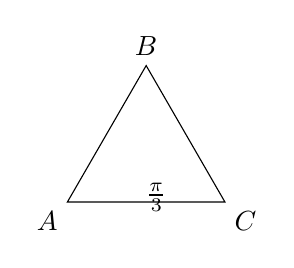
\begin{tikzpicture}
		\coordinate (A) at (-1,0);
		\coordinate (B) at (0, 1.732);
		\coordinate (C) at (1,0);

		\draw (A) node[below left]{$A$}
		-- (B) node[above]{$B$}
		-- (C) node[below right]{$C$}
		-- cycle;
		\tkzMarkAngle[size=0.8](C,A,B)
		\tkzLabelAngle [pos = 0.5](C,A,B){$\frac{\pi}{3}$}
		
		\tkzMarkAngle[size=0.8](B,C,A)
		
		\tkzMarkSegment[color=blue,pos=.5,mark=|](A,B)
		\tkzMarkSegment[color=blue,pos=.5,mark=|](B,C)  
	\end{tikzpicture}
\end{center}
Since we know the triangle is isosceles since $BC = AB$, we see that $\angle C = \frac{\pi}{3}$ radians. But that means that $\angle B = \frac{\pi}{3}$ radians as well (since the three internal angles must sum to $\pi$) and so the triangle is equilateral. Consequently every side has a length of 1, and so $AC = 1$. In fact the picture should look like the following.
\begin{center}
	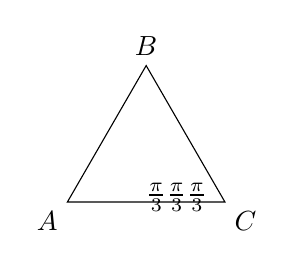
\begin{tikzpicture}
		\coordinate (A) at (-1,0);
		\coordinate (B) at (0, 1.732);
		\coordinate (C) at (1,0);

		\draw (A) node[below left]{$A$}
		-- (B) node[above]{$B$}
		-- (C) node[below right]{$C$}
		-- cycle;
		\tkzMarkAngle[size=0.6](C,A,B)
		\tkzLabelAngle [pos = 0.4](C,A,B){$\frac{\pi}{3}$}
		
		\tkzMarkAngle[size=0.6](B,C,A)
		\tkzLabelAngle [pos = 0.4](B,C,A){$\frac{\pi}{3}$}
		
		\tkzMarkAngle[size=0.6](A,B,C)
		\tkzLabelAngle [pos = 0.4](A,B,C){$\frac{\pi}{3}$}

		\tkzMarkSegment[color=blue,pos=.5,mark=|](A,B)
		\tkzMarkSegment[color=blue,pos=.5,mark=|](B,C)  
		\tkzMarkSegment[color=blue,pos=.5,mark=|](C,A)  
	\end{tikzpicture}
\end{center}
\item
In triangle $ABC$, $AB = 2$, $BC = 2$ and $AC = 3$. Find the angles of the triangle.
\newline
\begin{center}
	\begin{tikzpicture}
		\coordinate (A) at (-1.5,0);
		\coordinate (B) at (0, 1.732);
		\coordinate (C) at (1.5,0);

		\draw (A) node[below left]{$A$}
		-- (B) node[above]{$B$}
		-- (C) node[below right]{$C$}
		-- cycle;
		
		\tkzMarkSegment[color=blue,pos=.5,mark=|](A,B)
		\tkzMarkSegment[color=blue,pos=.5,mark=|](B,C) 

		\tkzLabelSegment[midway, sloped, above left](A,B){2}
		\tkzLabelSegment[midway, sloped, above right](B,C){2}
		\tkzLabelSegment[midway, below](A,C){3}
	\end{tikzpicture}
\end{center}
By the law of cosines we have
\[
9 = 8 -8\cos(\angle B),
\]
or equivalently
\[
\cos(\angle B) = -\frac{1}{8}.
\]
\[
\angle B \approx 1.696 \text{ radians}.
\]
Then since $\angle A = \angle C$ and the three angles sum to $\pi$, we have
\[
\angle A = \angle C \approx 0.723 \text{ radians}.
\]
\end{enumerate}

\subsubsection{Circles}
Find, for a sector of angle $\dfrac{\pi}{3}$ radians of a disc of radius 3:
\begin{enumerate}
\item the length of the permiter; and \item the area.
\end{enumerate}
\begin{enumerate}
\item
Since the sector has as an angle of $\frac{\pi}{3}$ it is a sixth of the circle. Consequently its arc length is
\[
\frac{1}{6}2\pi\times 3 = \pi.
\]
In addition, it has two sides that are radii and so have lengths of 3 each. Hence the perimter is $6 + \pi$.
\item 
Again, the area is a sixth and so is equal to
\[
\frac{1}{6}\times 9 \pi = \frac{3}{2}\pi \text{ units squared}.
\]
\end{enumerate}

\subsection{Sequences And Series}
\subsubsection{Arithmetic progressions}
An arithmetic progression has third term $\alpha$ and ninth term $\beta$. Find the sum to thirty terms. 
\newline
If the first term is $u$ and the common difference is $d$, then we have
\[
\alpha = u + 2d
\]
\[
\beta = u + 8d
\]
and the sum of the overall series is 
\[
15(2u + 29d) = 30u + 435d.
\]
We thus wish to write 
\[
a\alpha + b\beta = 30u + 435d.
\]
Expanding gives
\[
(a+b)u + (2a + 8b)d = 30 u + 435d. 
\]
We thus have a two variable system of equations:
\[
a+b = 30.
\]
\[
2a + 8b = 435.
\]
So
\[
b = \frac{125}{2}
\]
and
\[
a = \frac{-65}{2}.
\]
So we have that $\Sigma = -32.5 \alpha + 62.5 \beta$. 

\subsubsection{Binomial expansions}
Expand the following expressions, using the binomial expansion, as far as the fourth term:
\begin{enumerate}
\item $(1+x)^3$
\item $(2+x)^4$
\item $\left(2 + \frac{3}{x}\right)^5$.
\end{enumerate}
\begin{enumerate}
\item
\[
(1+x)^3 = 1 + 3x + 3x^2 + x^3.
\]
\item
\[
(2+x)^4 = 16 + 32x + 24x^2 + 8x^3 + (x^4).
\]
\item
\[
\left(2+ \frac{3}{x}\right)^5 = 32 + \frac{240}{x} + \frac{720}{x^2} + \frac{1080}{x^3} + \frac{810}{x^4} + \frac{243}{x^5}.
\]
\end{enumerate}

\subsubsection{Arithmetic and geometric progressions}
Prove that $\sum^N_1 n = \frac{1}{2}N(N+1)$.
\newline
Evaluate:
\begin{enumerate}
\item the sum of the odd integers from 11 to 99 inclusive.
\item $\sum_{n=1}^5(3n+2)$
\item $\sum^N_{n=0}(an+b)$ ($a$ and $b$ are constants)
\item $\sum_{r=0}^{10}2^r$
\item $\sum_{n=0}^N ar^{2n}$ ($a$ and $r$ are constants).
\end{enumerate}
\begin{proof}
We have
\[
\sum^N_{n=1} n = 1 + 2 + 3 + \hdots + N.
\]
This is a sum of $N$ terms. The mean of these terms, since they are consecutive numbers, is the middle term. That is half the $(N+1)^{\text{th}}$ term. So we have a sum of $N$ terms, which have a mean of $\frac{1}{2}(N+1)$. Hence their sum is the product of the mean and the number of terms:
\[
\frac{1}{2}N(N+1).
\]
\end{proof}
\begin{enumerate}
\item
\[
\sum_{n=0}^{44}11 + 2n = 45(55) = 2475.
\]
\item
\[
\sum^{5}_{n=1} (3n+2) = 5 + 8 + 11 + 14 + 17 + 20 = 75.
\]
\item
\[
\sum^{N}_{n=0}(an+b) = \frac{1}{2}(aN + 2b)(N).
\]
\item
\[
\sum_{r=0}^{10}2^r = 2^{11} - 1 = 2047.
\]
\item
\[
\sum^N_{n=0}ar^{2n} = \frac{a(r^{2N} - 1)}{r^2-1}.
\]
\end{enumerate}

\subsubsection{Iterative sequences}
The sequence $u_n$ satisfies $u_{n+1} = ku_n$ where $k$ is a fixed number, and $u_0 = 1$. Express $u_n$ in terms of $k$. Describe the behaviour of $u_n$ for large $n$ in the different cases that arise according to the value of $k$.
\newline
\[
u_{n+1} = ku_n.
\]
\[
u_0 = 1.
\]
\[
u_n = k^n.
\]
\begin{itemize}
\item
If $k > 1$, then $u_n \to \infty$.
\item
If $ k = 1$, then $u_n = 1$ for all $n$.
\item
If $0 < k < 1$ then $u_n \to 0$.
\item
If $k = 0$ then $u_n = 0$ , $n \neq 0$.
\item
If $-1 < k < 0$ then $u_n \to 0$.
\item
If $k = -1$ then $u_{2n} = 1$ and $u_{2n+1} = -1$. 
\item
If $k < -1$ then $u_{2n} \to \infty$ and $u_{2n+1} \to -\infty$.
\end{itemize}

\subsubsection{Binomial expansion for rational powers}
Find the first four terms in the expansions in ascending powers of $x$ of the following expressions, stating for what values of $x$ the expansion is valid in each case:
\begin{enumerate}
\item $(1+x)^{\frac{1}{2}}$
\item $(2+x)^{\frac{2}{5}}$
\item $\dfrac{(1+2x)^{\frac{1}{2}}}{(2+x)^{\frac{1}{3}}}$
\end{enumerate}
\begin{enumerate}
\item
\[
(1+x)^{\frac{1}{2}} \approx 1 + \frac{1}{2}x + \frac{1}{2!}\frac{1}{2}\cdot\frac{-1}{2}x^2 + \frac{1}{3!}\cdot\frac{1}{2}\cdot\frac{-1}{2}\cdot\frac{-3}{2}x^3
\]
\[
= 1 + \frac{1}{2}x - \frac{1}{8}x^2 + \frac{1}{16}x^3, |x| < 1.
\]
\item
\[
(2+x)^{\frac{2}{5}} = 2^{\frac{2}{5}}(1+\frac{x}{2})^{\frac{2}{5}} \approx 2^{\frac{2}{5}}\left(1 + \frac{2}{5}\cdot\frac{x}{2} + \frac{1}{2!}\cdot\frac{2}{5}\cdot\frac{-3}{5}\cdot\frac{x^2}{4} + \frac{1}{3!}\cdot\frac{2}{5}\cdot\frac{-3}{5}\cdot\frac{-8}{5}\cdot\frac{x^3}{8}\right), |x| < 2.
\]
\[
= 2^{\frac{2}{5}}\left(1 + \frac{1}{5}x - \frac{3}{100}x^2 + \frac{1}{125}x^3\right)
\]
\item
\[
\frac{(1+2x)^{\frac{1}{2}}}{(2+x)^{\frac{1}{3}}}
\]
\[
= (1+2x)^{\frac{1}{2}}(2+x)^{-\frac{1}{3}}
\]
\[
=2^{-\frac{1}{3}}\left(1+2x\right)^{\frac{1}{2}}\left(1+\frac{x}{2}\right)^{-\frac{1}{3}}
\]
\[
\approx 2^{-\frac{1}{3}}\left(1 + \frac{1}{2}2x + \frac{1}{2}\cdot\frac{1}{2}\cdot\frac{-1}{2}4x^2 + \frac{1}{3!}\cdot\frac{1}{2}\cdot\frac{-1}{2}\cdot\frac{-3}{2}8x^3\right)\times \hdots
\]
\[
\hdots \left(1 - \frac{1}{3}\cdot\frac{x}{2} + \frac{1}{2!}\cdot\frac{-1}{3}\cdot\frac{-4}{3}\cdot\frac{x^2}{4}+\frac{1}{3!}\cdot\frac{-1}{3}\cdot\frac{-4}{3}\cdot\frac{-7}{3}\frac{x^3}{8}\right)
\]
\[
=2^{-1\frac{1}{3}}\left(1 + x -\frac{1}{2}x^2 + \frac{1}{2}x^3\right)\left(1 - \frac{x}{6}+ \frac{x^2}{18}-\frac{7x^3}{324}\right)
\]
\[
2^{-\frac{1}{3}}\left(1 + \frac{5}{6}x -\frac{11}{18}x^2 + \frac{50}{81}x^3\right), |x| < \frac{1}{2}.
\]
\end{enumerate}

\subsubsection{Composition of approximations}
Given that, for small $\theta, \sin\theta \approx \theta - \frac{1}{6}\theta^3$ and $\cos \theta \approx 1 - \frac{1}{2}\theta^2$, find an approximation, ignoring powers of $\theta$ greater than 3, for $\sin(\frac{1}{2}\theta)\cos\theta + \sec 2\theta$.
\newline
Substituing the approximations, we obtain:
\[
\left(\frac{\theta}{2}-\frac{\theta^3}{48}\right)\left(1 - \frac{\theta^2}{2}\right) + (1 -2\theta^2)^{-1}
\]
\[
\approx \frac{\theta}{2} - \frac{13\theta^3}{48} + (1-2\theta^2)^{-1}
\]
\[
\approx \frac{\theta}{2} - \frac{13\theta^3}{48} + (1+2\theta^2)
\]
\[
= 1 + \frac{\theta}{2} + 2\theta^2 -\frac{13\theta^2}{48}.
\]


\subsection{Trigonometry}

\subsubsection{Solving trig equations}
Find the four values of $\theta$ in the range $0$ to $2\pi$ that satisfy the equation $2\sin^2\theta = 1$.
\[
2\sin^2\theta = 1
\]
\[
\sin^2\theta = \frac{1}{2}
\]
\[
\sin\theta = \pm \frac{\sqrt{2}}{2}
\]
\[
\theta = \pi/4, 3\pi/4, 5\pi/4, 7\pi/4.
\]

\subsubsection{Trig identities}
Prove that $\dfrac{\cot^2x+\sin^2x}{\cos x + \text{cosec } x} = \text{cosec } x - \cos x$.
\newline
We start by multiplying the right hand side by a carefully chosen form of 1 and proceed from there:
\[
(\text{cosec } x - \cos x)\frac{\text{cosec } x + \cos x}{\text{cosec } x + \cos x}
\]
\[
= \frac{\frac{1}{\sin^2x}-\cos^2x}{\text{cosec }x+ \cos x}
\]
\[
= \frac{\frac{1}{\sin^2x}-(1-\sin^2x)}{\text{cosec }x + \cos x }
\]
\[
= \frac{\frac{1-\sin^2x}{\sin^2x}+\sin^2x}{\text{cosec }x + \cos x}
\]
\[
= \frac{\cot^2x + \sin^2x}{\text{cosec }x + \cos x}.
\]

\subsubsection{Trig identities}
By writing $\dfrac{\pi}{12} = \dfrac{\pi}{3}- \dfrac{\pi}{4}$, use trigonometric identities to evaluate:
\begin{enumerate}
\item
$\cos \dfrac{\pi}{12}$
\item
$\sin \dfrac{\pi}{12}$
\item
$\cot \dfrac{\pi}{12}$
\end{enumerate}
\begin{enumerate}
\item
\[
\cos\frac{\pi}{12} = \cos\left(\frac{\pi}{3}-\frac{\pi}{4}\right)
\]
\[
=\cos\frac{\pi}{3}\cos\frac{\pi}{4}+\sin\frac{\pi}{3}\sin\frac{\pi}{4}
\]
\[
= \frac{1}{2}\cdot\frac{\sqrt{2}}{2}+\frac{\sqrt{3}}{2}\cdot\frac{\sqrt{2}}{2}
\]
\[
=\frac{\sqrt{6}+\sqrt{2}}{4}.
\]
\item
\[
\sin\frac{\pi}{12} = \sin\left(\frac{\pi}{3}-\frac{\pi}{4}\right)
\]
\[
=\sin\frac{\pi}{3}\cos\frac{\pi}{4} - \sin\frac{\pi}{4}\cos\frac{\pi}{3}
\]
\[
=\frac{\sqrt{3}}{2}\cdot\frac{\sqrt{2}}{2}-\frac{\sqrt{2}}{2}\cdot\frac{1}{2}
\]
\[
= \frac{\sqrt{6}-\sqrt{2}}{4}.
\]
\item
\[
\cot\frac{\pi}{12} = \frac{\cos\frac{\pi}{12}}{\sin\frac{\pi}{12}}
\]
\[
= \frac{\sqrt{6}+\sqrt{2}}{\sqrt{6}-\sqrt{2}}
\]
\[
= \frac{8+4\sqrt{3}}{4}
\]
\[
= 2 + \sqrt{3}.
\]
\end{enumerate}

\subsubsection{Trig identities}
If $t = \tan \frac{1}{2}\theta$, express the following in terms of $t$: 
\begin{enumerate}
\item
$\cos \theta$
\item
$\sin \theta$
\item
$\tan \theta$
\end{enumerate}
\begin{enumerate}
\item
We first note that
\[
t^2 + 1 = \frac{\sin^2\frac{\theta}{2}}{\cos^2\frac{\theta}{2}} + 1 = \frac{\sin^2\frac{\theta}{2} + \cos^2\frac{\theta}{2}}{\cos^2\frac{\theta}{2}} = \frac{1}{\cos^2\frac{\theta}{2}}.
\]
Hence
\[
\cos^2\frac{\theta}{2} = \frac{1}{1+t^2}.
\]
Then
\[
\cos\theta = 2\cos^2\frac{\theta}{2}-1
\]
\[
=\frac{2}{1+t^2}-1 
\]
\[
= \frac{1-t^2}{1+t^2}.
\]
\item
Similarly,
\[
\sin\theta = 2\sin\frac{\theta}{2}\cos\frac{\theta}{2}
\]
\[
= 2t\cos^2\frac{\theta}{2}
\]
\[
= \frac{2t}{1+t^2}.
\]
\item
Finally, from the tan double angle identity,
\[
\tan\theta = \frac{2t}{1-t^2}.
\]
\end{enumerate}


\subsubsection{Trig identities}
Simplify $\tan(\arctan \frac{1}{3} + \arctan \frac{1}{4})$.
\newline
We proceed via the tan sum-angle identity and obtain:
\[
\tan\left(\arctan\frac{1}{3}+\arctan\frac{1}{4}\right) = \frac{\frac{1}{3}+\frac{1}{4}}{1-\frac{1}{3}\cdot\frac{1}{4}}
\]
\[
=\frac{7}{11}.
\]

\subsubsection{Trig identities}
If $A, B$ and $C$ are the angles of a triangle, prove that
\[
\cos \left(\frac{B-C}{2} \right)-\sin\left(\frac{A}{2}\right) = 2 \sin\left(\frac{B}{2}\right)\sin\left(\frac{C}{2}\right).
\]
\newline
We first apply a compound angle identity backwards to to the right hand side to obtain
\[
2\sin\left(\frac{B}{2}\right)\sin\left(\frac{C}{2}\right) = \cos\left(\frac{B-C}{2}\right) - \cos\left(\frac{B+C}{2}\right).
\]
Since $A,B$ and $C$ are three internal angles in a triangle we know that $A+B+C = \pi$ and consequently $B+C = \pi - A$, which, when substituted gives us
\[
2\sin\left(\frac{B}{2}\right)\sin\left(\frac{C}{2}\right) = \cos\left(\frac{B-C}{2}\right) - \cos\left(\frac{\pi-A}{2}\right).
\]
But, $\cos\left(\frac{\pi}{2}-\theta\right) = \sin \theta$ and so $\cos\left(\frac{\pi-A}{2}\right) = \sin\left(\frac{A}{2}\right)$, which when substituted gives us, as desired,
\[
2\sin\left(\frac{B}{2}\right)\sin\left(\frac{C}{2}\right) = \cos \left(\frac{B-C}{2} \right)-\sin\left(\frac{A}{2}\right).
\]

\subsubsection{Solving trig equations}
Write $\sqrt{3}\sin\theta + \cos\theta$ in the form $A\sin(\theta + \alpha)$, where $A$ and $\alpha$ are to be determine.
\newline
Working backwards, we see
\[
A\sin(\theta + \alpha) = A(\sin\theta\cos\alpha + \sin\alpha\cos\theta).
\]
From here we equate coefficients and see that
\[
A\cos\alpha = \sqrt{3}
\]
\[
A \sin \alpha = 1.
\]
Dividing these two equations by each other yields
\[
\tan \alpha = \frac{1}{\sqrt{3}}
\]
and so one solution is 
\[
\alpha = \frac{\pi}{6}.
\]
From there we can substitute this into either of the equations to obtain
\[
A = 2.
\]
So
\[
\sqrt{3}\sin\theta + \cos\theta = 2\sin\left(\theta + \frac{\pi}{6}\right).
\]

\subsubsection{Solving trig equations}
Find the values of $\theta$ in the range $0$ to $2\pi$ which satisfy the equation
\[
\cos \theta + \cos 3\theta = \sin \theta + \sin 3\theta.
\]
We apply the compound angle identities repeatedly and obtain
\[
\cos \theta + \cos\theta\cos(2\theta) -\sin\theta\sin(2\theta) = \sin\theta + \sin\theta\cos(2\theta) + \sin(2\theta)\cos\theta
\]
\[
\iff \cos\theta + \cos\theta(\cos^2\theta-\sin^2\theta) -\sin\theta(2\sin\theta\cos\theta) = \sin\theta + \sin\theta(\cos^2\theta-\sin^2\theta) + \cos\theta(2\sin\theta\cos\theta)
\]
\[
\iff \cos \theta + \cos^3\theta -\cos\theta\sin^2\theta -2\sin^2\theta\cos\theta = \sin\theta + \cos^2\theta\sin\theta -\sin^3\theta + 2\cos^2\theta\sin\theta.
\]
Now we try and factor cleverly and look for where we can replace $1-\sin^2\theta$ with $\cos^2\theta$.
\[
\cos \theta(1 + \cos^2 \theta - \sin^2\theta -2\sin^2\theta) = \sin\theta + \cos^2\theta\sin\theta - \sin^3\theta + 2\cos^2\theta\sin\theta
\]
\[
\cos \theta(2\cos^2\theta-2\sin^2\theta) = \sin\theta(1 + \cos^2\theta - \sin^2\theta +2\cos^2\theta)
\]
\[
\cos \theta(2\cos^2\theta-2\sin^2\theta) = \sin\theta(4\cos^2\theta)
\]

Before we divide on both sides by $\cos \theta$, we must check if $\cos \theta$ could be equal to zero. If it were then $\theta = \frac{\pi}{2}$ or $\frac{3\pi}{2}$. If $\theta = \frac{\pi}{2}$, this would mean that $\cos\theta + \cos 3\theta = 0$ while $\sin\theta + \sin3\theta = 0$. Hence $\theta = \frac{\pi}{2}$ is a valid solution. Similarly, checking reveals that so too is $\frac{3\pi}{2}$. Now we can divide:

\[
2\cos^2\theta - 2\sin^2\theta = 4\sin\theta\cos\theta
\]
\[
2\cos(2\theta) = 2\sin(2\theta)
\]
\[
\cos(2\theta) = \sin(2\theta)
\]
\[
\tan(2\theta) = 1.
\]
Hence:
\[
\theta = \frac{\pi}{8}, \frac{\pi}{2}, \frac{5\pi}{8}, \frac{9\pi}{8}, \frac{3\pi}{2}, \frac{13\pi}{8}.
\]


\subsection{Vectors}

\subsubsection{Vectors in 3D}
Consider the four vectors
\[
\mathbf{A} = \begin{pmatrix} 16\\ -6 \\ 1 \end{pmatrix}, \quad \mathbf{B} = \begin{pmatrix} 4\\14\\-9 \end{pmatrix}, \quad \mathbf{C} = \begin{pmatrix} -15\\ 7\\ 4 \end{pmatrix}, \quad \mathbf{D} = \begin{pmatrix} 12\\12\\1 \end{pmatrix}.
\]
\begin{enumerate}
\item
Order the vectors by magnitude.
\item
Calculate the distance between the points with position vectors $\mathbf{A}$ and $\mathbf{B}$.
\end{enumerate}

\begin{enumerate}
\item
\[
|\mathbf{A}| = \left|\begin{pmatrix}
16\\
-6\\
1
\end{pmatrix}\right| = \sqrt{16^2 + 6^2 + 1^2}
\]
\[
= \sqrt{293}.
\]
\[
|\mathbf{B}| = \left| \begin{pmatrix}
4\\
14\\
-9
\end{pmatrix}\right| = \sqrt{4^2 + 14^2 + 9^2}
\]
\[
=\sqrt{293}.
\]
\[
|\mathbf{C}| = 
\left|\begin{pmatrix}
-15\\
7\\
4
\end{pmatrix}\right| = \sqrt{15^2 + 7^2 + 4^2}
\]
\[
= \sqrt{290}.
\]
\[
|\mathbf{D}| = 
\left|\begin{pmatrix}
12\\
12\\
1
\end{pmatrix}\right| = \sqrt{12^2 + 12^2 + 1^2}
\]
\[
= \sqrt{288}.
\]
Consequently
\[
|\mathbf{A}| = |\mathbf{B}| > |\mathbf{C}| > |\mathbf{D}|.
\]
\item
\[
|\mathbf{A - B}| = \left|\begin{pmatrix}
12\\
20\\
10
\end{pmatrix}\right| = \sqrt{12^2 + 20^2 + 10^2}
\]
\[
= \sqrt{644}.
\]
\end{enumerate}


\subsection{Differentiation}

\subsubsection{Stationary points}
Find the stationary points of the following functions, stating whether they are local maxima, minima or points of inflexion:
\begin{enumerate}
\item $y=x^2+2$
\item $y = x^3 - 3x+3$
\item $y = x^3 -3x^2 + 3x$ 
\item $y = x^3 + 3x + 3$.
\end{enumerate}
Sketch the graphs of the functions.
\newline
\begin{enumerate}
\item
\[
\frac{dy}{dx} = 2x.
\]
Consequently, this graph has a minimum at $(0,2)$.
\item
\[
\frac{dy}{dx} = 3x^2 - 3.
\]
Consequently this graph has turning points at 
\[
x = \pm 1.
\]
So there is a local maximum at $(-1, 5)$ and a local minimum at $(1,1)$.
\item
\[
\frac{dy}{dx} = 3x^2 -6x +3.
\]
Consequently this graph has turning points at
\[
x = 1\pm\sqrt{36-36} .
\]
Hence this graph has its only turning point at $(1,1)$. The second derivative
\[
y''(1) = 6(1) - 6 = 0
\]
and so this is an inflexion point (which was expected since its the only turning point in a cubic anyway).
\item
\[
\frac{dy}{dx} = 3x^2 + 3.
\]
Since the derivative is strictly positive (from the trivial inequality), there are no turning points in this graph.
\end{enumerate}
\begin{center}
\includegraphics[scale = 0.1]{media/Sketching_from_derivatives}
\end{center}

\subsubsection{Differentiation from first principles}
Calculate the derivative of $y = x^2 + 1$ from first principles (i.e. by considering the derivative of a function as the limit of the gradient of a chord).
\newline
We do as requested and note that the gradient would be given by the change in $y$ over the change in $x$ where we let the change in $x$ tend very small.
\[
\frac{dy}{dx} = \lim_{h \to 0} \frac{[(x+h)^2 + 1] - (x^2 + 1)}{h}
\]
\[
= \lim_{h \to 0} \frac{2xh+h^2}{h}
\]
\[
= \lim_{h \to 0} 2x + h
\]
\[
= 2x.
\]

\subsubsection{Chain rule and product rule}
Using the chain and product rules etc., find the derivatives of:
\begin{enumerate}
\item $y = \sin(x^2)$
\item $y = a^x\text{(hint: take logs)}$
\item $y = \ln(x^a + x^{-a})$
\item $y = x^x$
\item $y = \sin^{-1}x$
\end{enumerate}
where $a$ is a positive constant.

\begin{enumerate}
\item
\[
\frac{dy}{dx} = 2x\cos x^2 
\]
\item
\[
\frac{d}{dx}a^x = \frac{d}{dx}e^{x\ln a} = a^x \ln a.
\]
\item
\[
\frac{dy}{dx} = \frac{ax^{a-1} -ax^{-a-1}}{x^a + x^{-a}}
\]
\item
\[
y = x^x. 
\]
\[
\ln y = x \ln x 
\]
\[
\frac{1}{y}\frac{dy}{dx} = \ln x + 1
\]
\[
\frac{dy}{dx} = \ln(x)x^x + x^x.
\]
\item
\[
\sin y = x 
\]
\[
\cos y \frac{dy}{dx} = 1
\]
\[
\frac{dy}{dx} = \frac{1}{\cos{y}}
\]
\[
= \frac{1}{\sqrt{1-x^2}}.
\]
\end{enumerate}

\subsubsection{Implicit differentiation}
\input{Implicit_differentiation_1.tex}

\subsubsection{Implicit differentiation}
\input{Implicit_differentiation_2.tex}


\subsection{Integration}

\subsubsection{Integration techniques}
Find the following indefinite integrals (stating the values of $x$ for which the integrand is a real function):
\begin{enumerate}
\item $\int \dfrac{1}{2+x^2} \text{ }dx$ (set $x = \sqrt{2}\tan\theta$)
\item $\int \dfrac{1}{\sqrt{3+2x-x^2}} \text{ }dx$ (set $x-1 = 2\sin\theta$)
\item $\int \dfrac{1}{x\sqrt{1-x}} \text{ }dx$ 
\item $\int \ln x \text{ }dx$.
\end{enumerate}
\begin{enumerate}
\item
\[
I = \int \frac{1}{2+x^2}dx.
\]
Let $x = \sqrt{2}\tan\theta$ so $dx = \sqrt{2}$sec$^2\theta d\theta$. Then
\[
I = \int \frac{\sqrt{2}\sec^2\theta}{2+2\tan^2\theta}d\theta
\]
\[
= \int \frac{\sqrt{2}}{2\cos^2\theta + 2\sin^2\theta}d\theta
\]
\[
= \int \frac{\sqrt{2}}{2}d\theta
\]
\[
= \frac{\sqrt{2}}{2}\theta
\]
\[
=\frac{\sqrt{2}}{2} \arctan{\frac{x}{\sqrt{2}}} + C.
\]
\item
\[
I = \int \frac{1}{\sqrt{3+2x-x^2}}dx
\]
Let $x-1 = 2\sin\theta$ so $dx = 2\cos\theta d\theta$.
\[
I = \int \frac{1}{\sqrt{-(x-1)^2 +4}}
\]
\[
I = \int \frac{2\cos\theta}{\sqrt{-4\sin^2\theta+4}}d\theta
\]
\[
= \int \frac{\cos\theta}{\sqrt{1-\sin^2\theta}}d\theta
\]
\[
= \int d\theta
\]
\[
= \theta
\]
\[
= \arcsin\frac{x-1}{2}.
\]
\item
\[
I = \int \frac{1}{x\sqrt{1-x}}dx.
\]
Let $u = \sqrt{1-x}$ so $x = 1-u^2$ and $du = \frac{-1}{2u}$. Then
\[
I = \int\frac{2u}{u(1-u^2)}du 
\]
\[
= 2 \int\frac{1}{1-u^2}du.
\]
Now we try to use partial fractions and write
\[
\frac{1}{1-u^2} = \frac{A}{1+u} + \frac{B}{1-u}.
\]
Hence 
\[
1 = A - uA + B + uB.
\]
So $A - B = 0$ and $A + B = 1$. Hence 
\[
\frac{1}{1-u^2} = \frac{1}{2(1+u)} + \frac{1}{2(1-u)}.
\]
Hence
\[
I = \int \frac{1}{1+u} + \frac{1}{1-u}du
\]
\[
= \ln|1+u| - \ln|1-u| + C 
\]
\[
= \ln|1 + \sqrt{1-x}| - \ln|1 - \sqrt{1-x}| + C.
\]
\item
\[
I = \int \ln x dx.
\]
Let $u = \ln x$ so $u' = 1/x$ and let $v' = 1$ so $v = x$. Then applying the integration by parts formula,
\[
I = x\ln x - \int dx
\]
\[
= x\ln x - x + C.
\]
\end{enumerate}

\subsubsection{Integration techniques}
Evaluate the following definite integrals:
\begin{enumerate}
\item $\int^L_0 xe^{-x} \text{ }dx$
\item $\int^{\pi/2}_0 \sin3\theta \cos\theta \text{ }d\theta$
\item $\int^1_0 \dfrac{x^2+1}{x^3+3x+2}\text{ d}x$
\item $\int^{\pi/2}_0 \dfrac{1}{3+5\cos\theta} \text{ }d\theta$ [use $t = \tan(\frac{1}{2}\theta)$].
\end{enumerate}
In part 1, can you suggest what happens as $L \to \infty$.
\begin{enumerate}
\item
First we define
\[
I(L) = \int^L_0 xe^{-x} dx.
\]
Then, by parts, let $u = x$ and $v' = e^{-x}$ so $u' = 1$ and $v = -e^{-x}$ and
\[
I(L) = -xe^{-x}\rvert^L_0 + \int^L_0 e^{-x} dx 	
\]
\[
= (-xe^{-x})\rvert^L_0 + (-e^{-x})\rvert^L_0
\]
\[
= -Le^{-L} - e^{-L} +1
\]
\[
-e^{-L}(L+1) + 1.
\]
As $L \to \infty$, $I(L) \to 1$.
\item
First we define
\[
I = \int^{\pi/2}_0 \sin3\theta\cos\theta d\theta.
\]
Then, by parts, let $u = \sin 3\theta$ and $v' = \cos\theta$ so $u' = 3\cos3\theta$ and $v = \sin\theta$. Then
\[
I = (\sin\theta\sin3\theta)\rvert^{\pi/2}_0 - 3\int \sin\theta\cos3\theta d\theta.
\]
Now, by parts, let $x = \cos 3\theta$ and $y' = \sin \theta$ so that $x' = -3\sin3\theta$ and $y = -\cos\theta$. Then
\[
I = (\sin\theta\sin3\theta)\rvert^{\pi/2}_0 -3(-\cos\theta\cos3\theta - 3\int^{\pi/2}_0 \cos\theta\sin3\theta d\theta)
\]
\[
I = (\sin\theta\sin3\theta)\rvert^{\pi/2}_0 + (3\cos\theta\cos3\theta)\rvert^{\pi/2}_0 + 9I
\]
\[
-8I = (\sin\theta\sin3\theta)\rvert^{\pi/2}_0 + (3\cos\theta\cos3\theta)\rvert^{\pi/2}_0
\]
\[
= (-1 + 0) - (0 + 3)
\]
\[
= -4.
\]
\[
I = \frac{1}{2}.
\]
\item
First we define
\[
I = \int^1_0 \frac{x^2+1}{x^3+3x+2} dx.
\]
Let $u = x^3 + 3x+ 2$ so that $du = dx(3x^2 + 3)$.
Then 
\[
I = \int^6_2 \frac{x^2+1}{u(3x^2+3)} du 
\]
\[
= \int^6_2 \frac{1}{3u}du
\]
\[
= (\frac{1}{3}\ln u)\rvert^6_2
\]
\[
= \frac{1}{3}\ln3.
\]
\item
First we define
\[
I = \int^{\pi/2}_0 \frac{1}{3+5\cos\theta}\text{ }d\theta.
\]
Then we use the standard $t$-substitution. That is, $t = \tan(\frac{1}{2}\theta)$ so $d\theta = \cos^2(\frac{1}{2}\theta)dt$. This gives us
\[
I = \int^1_0 \frac{1}{3 + \frac{5-5t^2}{1+t^2}}\cdot\frac{2}{1+t^2}\text{ }dt
\]
\[
= \int^1_0 \frac{2}{3+3t^2 + 5 - 5t^2}\text{ }dt
\]
\[
= \int^1_0 \frac{2}{8-2t^2}\text{ }dt
\]
\[
=\int^1_0 \frac{1}{4-t^2}\text{ }dt
\]
\[
=\frac{1}{4}\int^1_0 \frac{1}{2+t}\text{ dt} + \frac{1}{4}\int^1_0 \frac{1}{(2-t)}\text{ }dt
\]
\[
=\frac{1}{4}\left(\ln3\right).
\]
\end{enumerate}


\subsection{Differential equations}

\subsubsection{Seperable first order ODEs}
Solve the following differential equation:
\[
x\frac{dy}{dx} + (1-y^2) = 0; \quad \quad y = 0 \text{ when } x = 1.
\]
\newline
\[
x\frac{dy}{dx}+ (1-y^2) = 0; (1,0)
\]
\[
x\frac{dy}{dx} = y^2 - 1
\]
\[
\int \frac{1}{x}dx = \int \frac{1}{y^2-1}dy
\]
\[
\int \frac{1}{x}dx = \frac{1}{2}\int \frac{1}{y-1}dy - \frac{1}{2}\int\frac{1}{y+1}dy
\]
\[
\ln x + C =  \frac{1}{2}\ln|y-1| - \frac{1}{2}\ln|y+1|
\]
\[
Cx = \sqrt{\frac{|y-1|}{|y+1|}}.
\]
When $x = 1$, $y = 0$. So
\[
C = \sqrt{\frac{1}{1}} = 1.
\]
\[
C = 1.
\]
\[
x = \sqrt{\frac{|y-1|}{|y+1|}}.
\]
\[
x^2 = \frac{|y-1|}{|y+1|}
\]
\[
x^2y + x^2 = y - 1
\]
\[
x^2 + 1 = y - x^2y
\]
\[
y = \frac{1+x^2}{1-x^2}.
\]


\section{Further Mathematics}


\subsection{Complex mathematics}

\subsubsection{Basic manipulations}
\begin{enumerate}
\item
Determine the real and imaginary parts of 
\[
\frac{1+i}{2-i}.
\]
\item
Find the roots of the quadratic equation $z^2 -2z + 2 = 0$. Determine the modulus and argument of each root. Plot the roots of an Argand diagram.
\end{enumerate}
\begin{enumerate}
\item
\[
z = \frac{1+i}{2-i}\cdot\frac{2+i}{2+i} = \frac{(1+i)(2+i)}{5}.
\]
Hence 
\[
\text{Re}(z) = \frac{1}{5}. 
\]
\[
\text{Im}(z) = \frac{3}{5}.
\]
\item
\[
z = 1 \pm i. 
\]
The arguments are $\pi/4$ (positive) and $-\pi/4$ (negative) and the modulus of both is $\sqrt{2}$ so they lie on a circle of radius $\sqrt{2}$ centered at the origin.
\begin{center}
	\begin{tikzpicture}
		\draw [->] (-3.5,0) -- (3.5,0) node [above left]  {$\Re\{z\}$};
		\draw [->] (0,-3.5) -- (0,3.5) node [below right] {$\Im\{z\}$};
		\draw (0,0) circle (1.414);
		\node at (1,1) {\textbullet};
		\node at (1,-1) {\textbullet};
		\foreach \n in {-2,-1,1,2,}{%
			\draw (\n,-3pt) -- (\n,3pt)   node [above] {$\n$};
			\draw (-3pt,\n) -- (3pt,\n)   node [left] {$\n i$};
			}
	\end{tikzpicture}
\end{center}
\begin{center}
	\begin{tikzpicture}
		\draw [->] (-3.5,0) -- (3.5,0) node [above left]  {$\Re\{z\}$};
		\draw [->] (0,-3.5) -- (0,3.5) node [below right] {$\Im\{z\}$};
		\draw (0,0) circle (1.414);
		\node at (1,1) {\textbullet};
		\node at (1,-1) {\textbullet};
		\foreach \n in {-2,-1,1,2,}{%
			\draw (\n,-3pt) -- (\n,3pt)   node [above] {$\n$};
			\draw (-3pt,\n) -- (3pt,\n)   node [left] {$\n i$};
			}
	\end{tikzpicture}
\end{center}
\end{enumerate}

\subsubsection{Further properties}
\begin{enumerate}
\item
Use de Moivre's theorem to express $\cos 5\theta$ in terms of powers of $\sin\theta$ and $\cos \theta$.
\item
Sketch the loci $|z-i| = 2$ and $|z+i| = |z-2|$.
\end{enumerate}
\begin{enumerate}
\item
\[
\text{Re}(e^{5i\theta}) = \text{Re}((\text{cis}\theta)^5) 
\]
\[
=\cos^5\theta -10\cos^3\theta\sin^2\theta + 5\cos\theta\sin^4\theta.
\]
\item
\[
|z-i| = 2
\]
\begin{tikzpicture}
	\draw [->] (-5,0) -- (5,0) node [above left]  {$\Re\{z\}$};
	\draw [->] (0,-5) -- (0,5) node [below right] {$\Im\{z\}$};
	\draw (0,1) circle (2);
	\foreach \n in {-5,...,-1,1,2,...,5}{%
			\draw (\n,-3pt) -- (\n,3pt)   node [above] {$\n$};
			\draw (-3pt,\n) -- (3pt,\n)   node [left] {$\n i$};
			}
\end{tikzpicture}
\newpage
\[
|z+i| = |z-2|
\]
\begin{tikzpicture}
	\draw [->] (-5,0) -- (5,0) node [above left]  {$\Re\{z\}$};
	\draw [->] (0,-5) -- (0,5) node [below right] {$\Im\{z\}$};
	\draw (-1.75,5) -- (3.25,-5);
	\foreach \n in {-5,...,-1,1,2,...,5}{%
			\draw (\n,-3pt) -- (\n,3pt)   node [above] {$\n$};
			\draw (-3pt,\n) -- (3pt,\n)   node [left] {$\n i$};
			}
\end{tikzpicture}
\end{enumerate}



\subsection{Vectors}

\subsubsection{Vector equation of lines}
Show that the points with position vectors
\[
\begin{pmatrix}1\\ 0\\ 1 \end{pmatrix}, \quad \begin{pmatrix} 2\\ 1 \\ 0 \end{pmatrix}, \quad \begin{pmatrix} 0 \\ -1 \\ 2 \end{pmatrix}
\]
lie on a straight line and give the equation of the line in the form $\mathbf{r} = \mathbf{a} + \lambda\mathbf{b}$.
\newline
\[
\mathbf{a} = \begin{pmatrix}
1 \\
0 \\
1
\end{pmatrix}, \mathbf{b} = \begin{pmatrix}
2\\
1\\ 
0
\end{pmatrix} \mathbf{c} = \begin{pmatrix}
0\\
-1\\
2
\end{pmatrix}.
\]
\[
\mathbf{a} - \mathbf{b} = \begin{pmatrix}
-1\\
-1\\
1
\end{pmatrix}; \quad \mathbf{b} - \mathbf{c} = \begin{pmatrix}
2\\
2\\
-2
\end{pmatrix} = -2(\mathbf{a} - \mathbf{b}).
\]
Since the line segments joining A and B and joining B and C are scalar multiples of each other and both go through point $B$ with position vector $\mathbf{b}$, the three points are colinear, lying on the line $\mathbf{r} = \begin{pmatrix} 0\\-1\\2 \end{pmatrix} + \lambda \begin{pmatrix} 1\\1\\-1 \end{pmatrix}$.


\subsection{Matrices}

\subsubsection{Basic properties}
Calculate $\mathbf{A} + \mathbf{B}$, $\mathbf{AB}$ and $\mathbf{BA}$ for
\[
\mathbf{A} = \begin{bmatrix} 1 & 2\\ 3 & 4 \end{bmatrix} \quad \quad \mathbf{B} = \begin{bmatrix} -2 & -1 \\ 4 & 2 \end{bmatrix}.
\]
\newline
\[
\mathbf{A} + \mathbf{B} = \begin{bmatrix}
-1 & 1\\
7 & 6
\end{bmatrix}.
\]
\[
\mathbf{AB} = \begin{bmatrix}
6 & 3\\
10 & 5
\end{bmatrix}; \mathbf{BA} = \begin{bmatrix}
-5 & -8\\
10 & 16
\end{bmatrix}.
\]

\subsubsection{Non-commutativity}
Find matrices $\mathbf{A}$ and $\mathbf{B}$ such that $\mathbf{AB}= 0$ and $\mathbf{BA} \neq 0$.
\newline
An example of two such matrices is
\[
\mathbf{A} = \begin{bmatrix}
0 & 1\\
0 & 1
\end{bmatrix},\quad \mathbf{B} = \begin{bmatrix}
1 & 1\\
0 & 0
\end{bmatrix}.
\]

\subsubsection{Transformations}
A linear transformation is described by the matrix
\[
\begin{bmatrix} 1 & -1 \\ 1 & 1 \end{bmatrix}.
\]
Show that this transformation is the composition of a rotation and a scaling.
\newline
Note that
\[
\begin{bmatrix}
1 & -1\\
1 & 1
\end{bmatrix} = \begin{bmatrix} \sqrt{2} & 0\\
0 & \sqrt{2} \end{bmatrix}
\begin{bmatrix}
\frac{1}{\sqrt{2}} & \frac{-1}{\sqrt{2}}\\
\frac{1}{\sqrt{2}} & \frac{1}{\sqrt{2}}
\end{bmatrix}
\]
and so this is the composition of scaling by factor $\sqrt{2}$ and rotating $\pi/4$ radians.


\subsection{Series}

\subsubsection{Summation of series}
Sum the following series
\[
\sum^n_{r=1} r^2 \quad \quad \sum^n_{r=1} r(r^2+2).
\]
\newline
\[
\sum^n_{r=1} r^2 = \frac{n(n+1)(2n+1)}{6}
\]
\[
\sum^n_{r=1} r(r^2 +2) = \frac{n^4 + 5n^3 + 2n^2 + n}{4}
\]

\subsubsection{Method of differences}
Use partial fractions to sum the series
\[
\sum^n_{r=1} \frac{1}{r(r+1)}.
\]
\newline
\[
\frac{1}{r(r+1)} = \frac{A}{r+1} + \frac{B}{r}.
\]
So $Ar + Br + B = 1$. Hence $A+B= 0$ and $B = 1$. So $A = -1$. So
\[
\frac{1}{r(r+1)} = \frac{1}{r} - \frac{1}{r+1}
\]
and so 
\[
\sum^n_{r=1} \frac{1}{r(r+1)} = (\frac{1}{1} - \frac{1}{2}) + (\frac{1}{2} - \frac{1}{3}) + (\frac{1}{3} - \frac{1}{4}) + \hdots + -\frac{1}{n+1}
\]
which telescopes and so
\[
= 1 - \frac{1}{n+1}
\]
\[
= \frac{n}{n+1}.
\]


\subsection{Mathematical induction}

\subsubsection{Sequences}
If $a_{n+1} = 3a_n + 4$ and $a_1 = 1$ then deduce a formula for $a_n$ for any $n \geq 1$. Use mathematical induction to prove your result.
\newline
Computing a few values gives
\[
a_2 = 7
\]
\[
a_3 = 25
\]
\[
a_4 = 79
\]
It looks like $a_n = 3^n - 2$. Hence let $P(n)$ be the statement that $a_n = 3^n -2$. $P_1$ is true since $a_1 = 1 = 3^1 - 2.$ Now assume $P(k)$ is true for some natural $k$. Now consider $P(k+1)$. 
\[
a_{k+1} = 3(a_k) + 4
\]
but since $P(k)$ has been assumed to be true that means
\[
a_{k+1} = 3(3^k -2)+4 = 3^{k+1} - 6 + 4 = 3^{k+1} -2.
\]
Hence $P(k+1)$ is also true. Since $P(k)$ implies $P(k+1)$ and since $P(1)$ is true, by mathematical induction, $P(n)$ is true for all natural $n \geq 1$. 

\subsubsection{Integration}
Use mathematical induction to prove that, for a non-negative integer $n$, 
\[
\int^\infty_0 x^ne^{-x} dx = n!.
\]
\newline
Let $P(n)$ be the statement that $\int^{\infty}_0 x^ne^{-x}dx = n!$. $P(0)$ is true since 
\[
\int^\infty_0 e^{-x} dx = -e^{-x}\rvert^\infty_0 = 0 - (-1) = 1 = 0!.
\]
Now assume $P(k)$ is true for some natural $k$. Now consider $P(k+1)$. We are interested in computing
\[
\int^{\infty}_0 x^{k+1}e^{-x}dx.
\]
By parts, let $u = x^{k+1}$ so $u' = (k+1)x^k$ and let $v' = e^{-x}$ so $v = -e^{-x}$. Then
\[
\int^{\infty}_0 x^{k+1}e^{-x}dx = (-x^{k+1}e^{-x})\rvert^\infty_0 + (k+1)\int^\infty_0 x^ke^{-x}dx.
\]
But since we have assumed $P(k)$ is true, this means that this can be simplified to
\[
= (-x^{k+1}e^{-x})\rvert^\infty_0 + (k+1)k! = 0 + (k+1)k!
\]
\[
= (k+1)!.
\]
Hence $P(k+1)$ is true if $P(k)$ is true. Since $P(k)$ implies $P(k+1)$ and since $P(0)$ is true, $P(n)$ is true for all non-negative integers $n$ by mathematical induction.


\subsection{Hyperbolic functions}

\subsubsection{Basic properties}
State the definitions of sinh $x$ and cosh $x$. Prove that
\[
\text{cosh}^2x - \text{sinh}^2x = 1 \quad \quad \quad \text{sinh}2x = 2 \text{sinh}x\text{cosh}x
\]
\newline
$\sinh x$ is the odd part of the exponential function and $\cosh x$ is the even part. We thus have
\[
\sinh x = \frac{e^x-e^{-x}}{2}
\]
\[
\cosh x = \frac{e^x + e^{-x}}{2}.
\]
A simplie computation reveals
\[
\cosh^2x - \sinh^2x = (\cosh x - \sinh x)(\cosh x + \sinh x)
\]
\[
e^{-x}e^x = 1.
\]
Similarly,
\[
2\sinh x\cosh x = 2\left(\frac{e^x+e^{-x}}{2}\right)\left(\frac{e^x-e^{-x}}{2}\right) 
\]
\[
= \frac{(e^x+e^{-x})(e^x -e^{-x})}{2}
\]
\[
= \frac{e^{2x} -e^{-2x}}{2} = \sinh 2x.
\]

\subsubsection{Differentiation}
Prove that
\[
\frac{d}{dx}\text{tanh}x = \text{sech}^2x.
\]
\newline
\[
\tanh x = \frac{\sinh x}{\cosh x}
\]
\[
= \frac{e^x -e^{-x}}{e^x+e^{-x}}.
\]
\[
\frac{d}{dx}\tanh x = \frac{d}{dx}(e^x-e^{-x})(e^x+e^{-x})^{-1}
\]
\[
= (e^x +e^{-x})(e^x+e^{-x})^{-1} + (e^x-e^{-x})-1(e^x +e^{-x})^{-2}(e^{x} -e^{-x})
\]
\[
=\frac{e^x + e^{-x}}{e^x + e^{-x}} - \frac{(e^x-e^{-x})(e^x-e^{-x})}{(e^x+e^{-x})^2}
\]
\[
=\frac{(e^x+e^{-x})^2 -(e^x-e^{-x})^2}{(e^x+e^{-x})^2}
\]
\[
= \frac{[(e^x + e^{-x}) + (e^x-e^{-x})][(e^x+e^{-x})-(e^x-e^{-x})]}{(e^x+e^{-x})^2}
\]
\[
= \frac{(2e^x)(2e^{-x})}{(e^x+e^{-x})^2}
\]
\[
= \frac{4}{(e^{x}+e^{-x})^2}
\]
\[
= \frac{1}{(\frac{e^x+e^{-x}}{2})^2}
\]
\[
= \frac{1}{\cosh^2x}
\]
\[
= \text{sech}^2x.
\]
\end{document}